\begin{figure}[p]
  \centering
    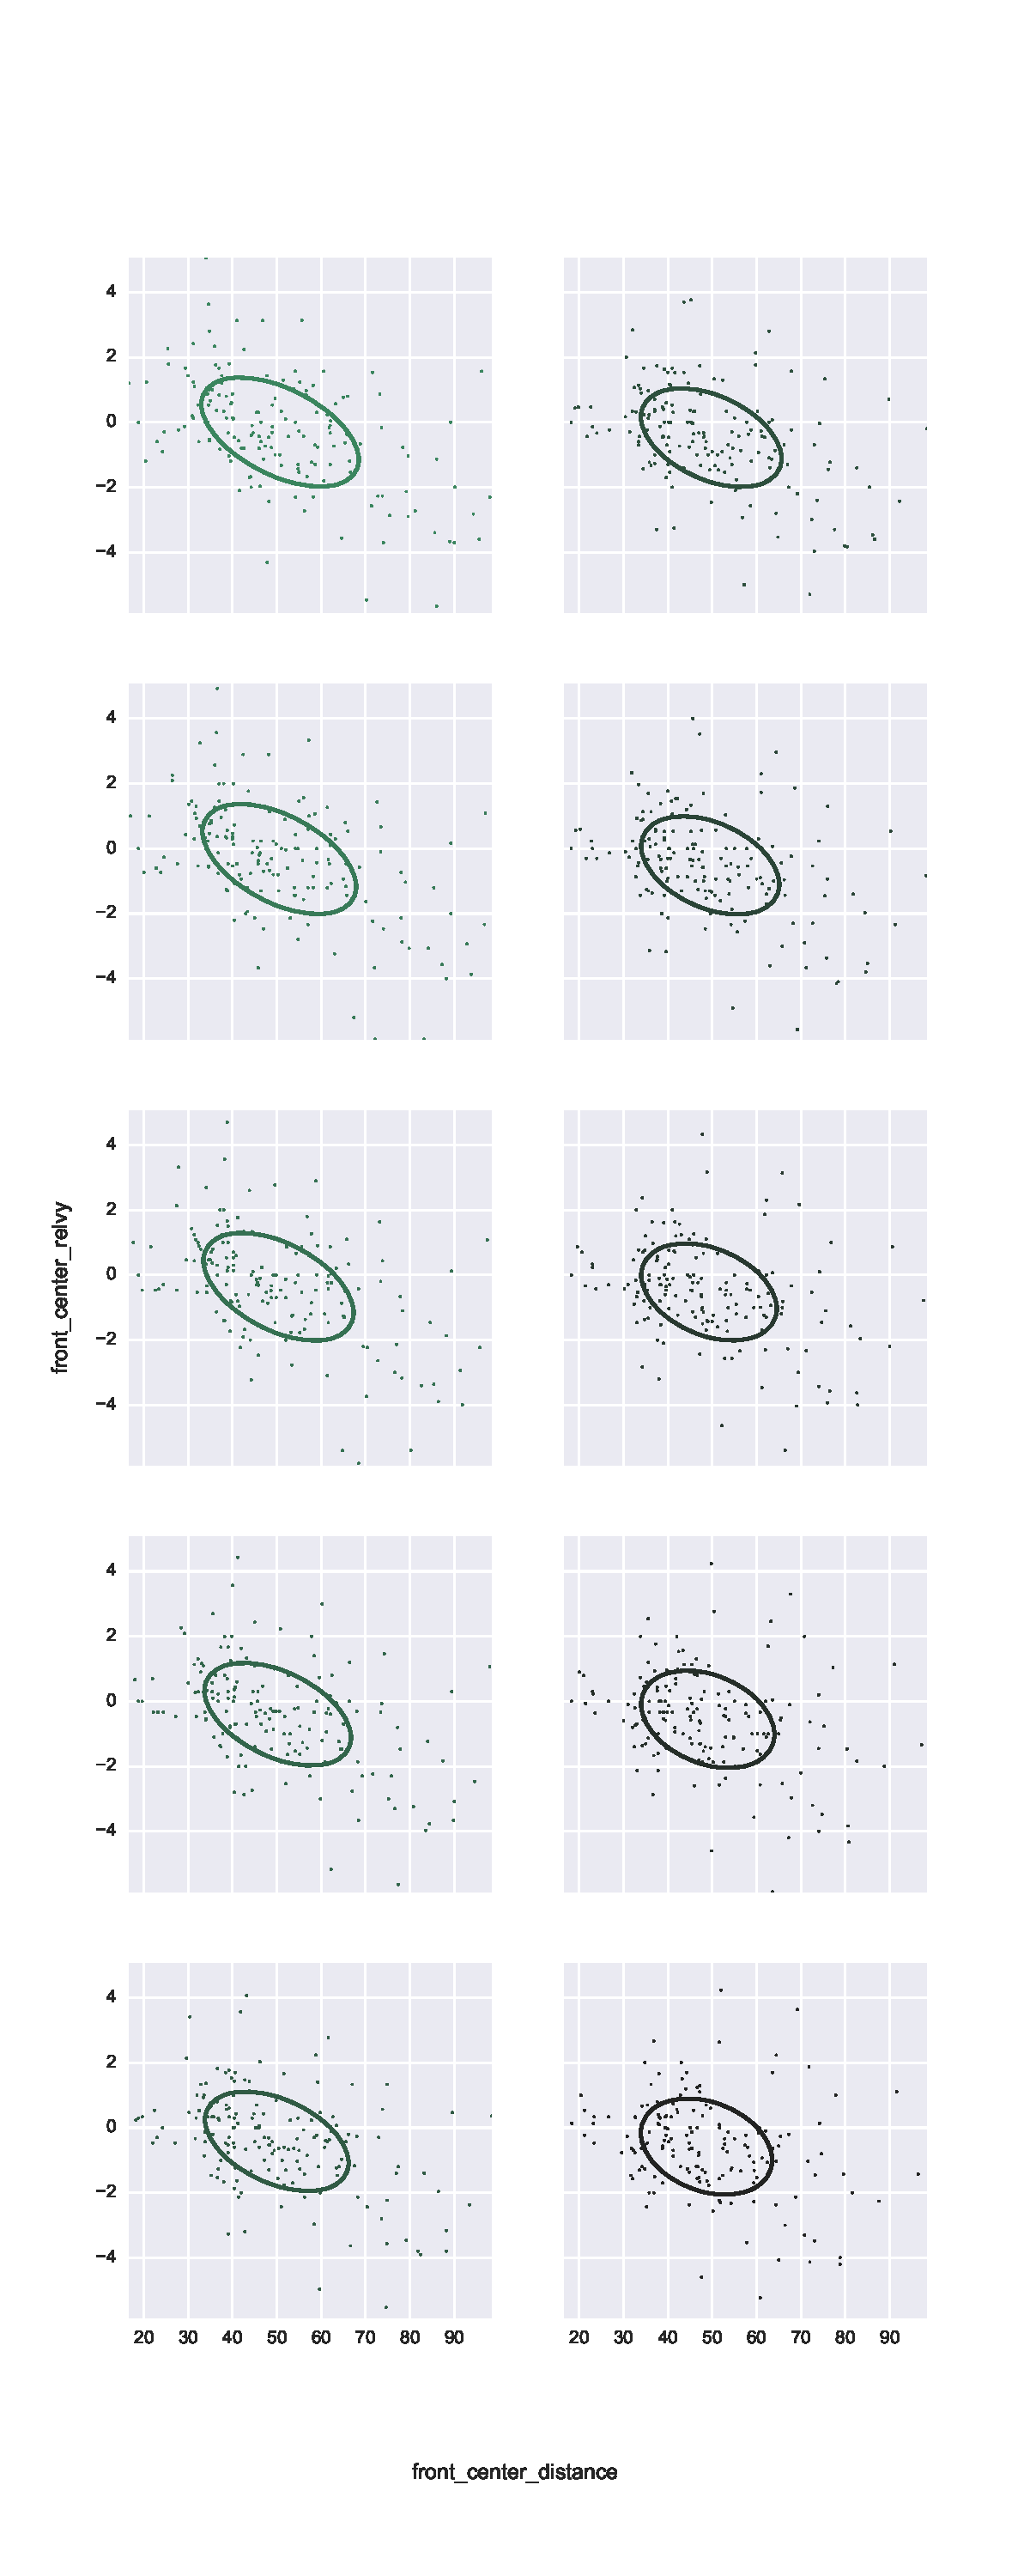
\includegraphics[width=11cm,keepaspectratio]{fig/scatter_ellipse_front_center_distance_front_center_relvy0.pdf}
  % \caption{車線変更開始10秒前から7.5秒前の時点における先行車両との相対距離と相対速度を,すべてのデータにおいてプロットした散布図.また,これを正規分布で近似し,長軸,短軸を標準偏差とした楕円.x軸が距離を,y軸が速度を表す.}
  % \label{fig:scatter_ellipse0}
\end{figure}
\begin{figure}[p]
  \centering
    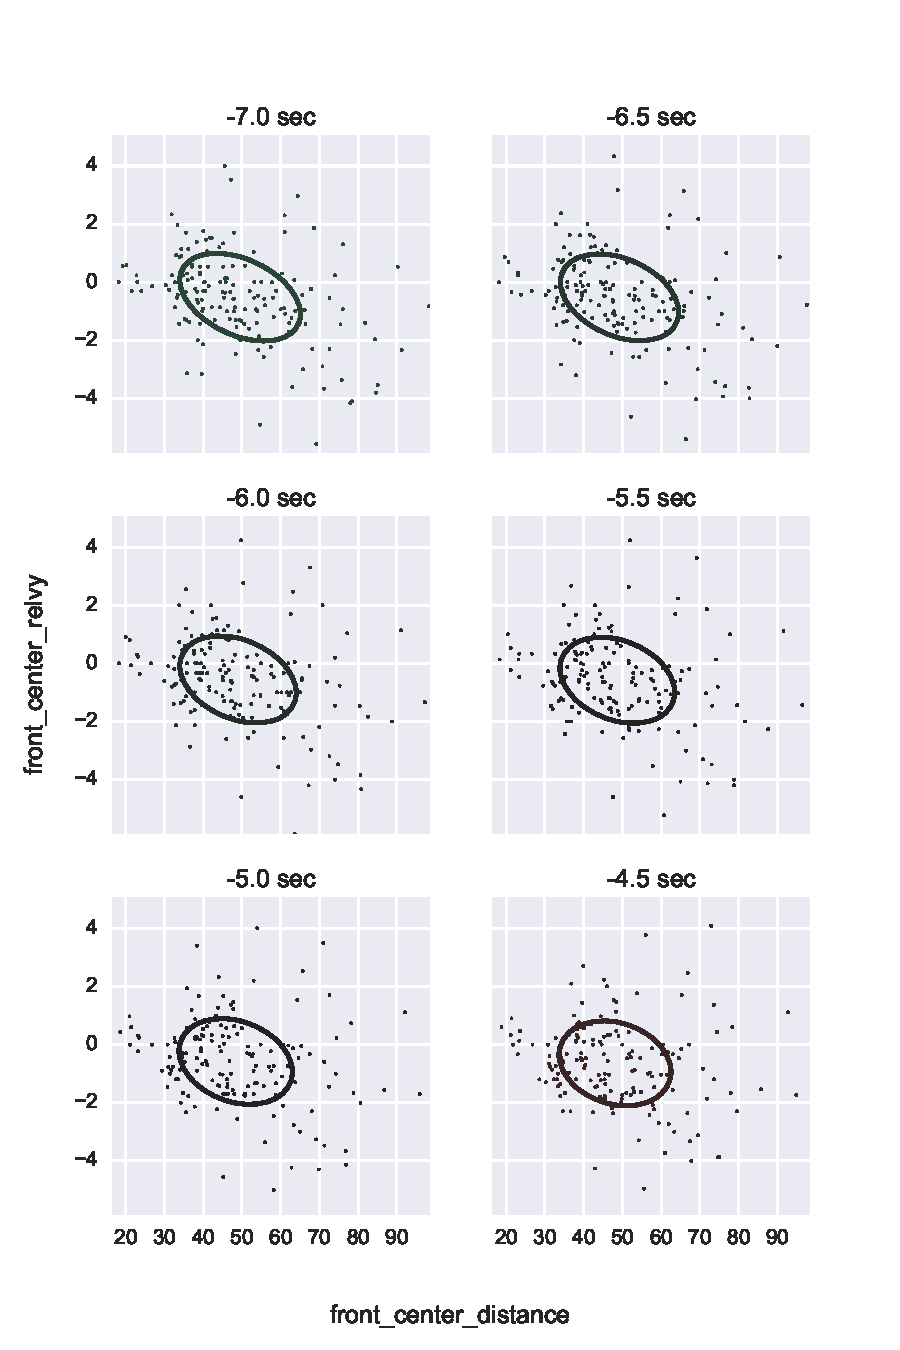
\includegraphics[width=11cm,keepaspectratio]{fig/scatter_ellipse_front_center_distance_front_center_relvy1.pdf}
  % \caption{車線変更開始7秒前から4.5秒前の時点における先行車両との相対距離と相対速度を,すべてのデータにおいてプロットした散布図.また,これを正規分布で近似し,長軸,短軸を標準偏差とした楕円.x軸が距離を,y軸が速度を表す.}
  % \label{fig:scatter_ellipse1}
\end{figure}
\begin{figure}[p]
  \centering
    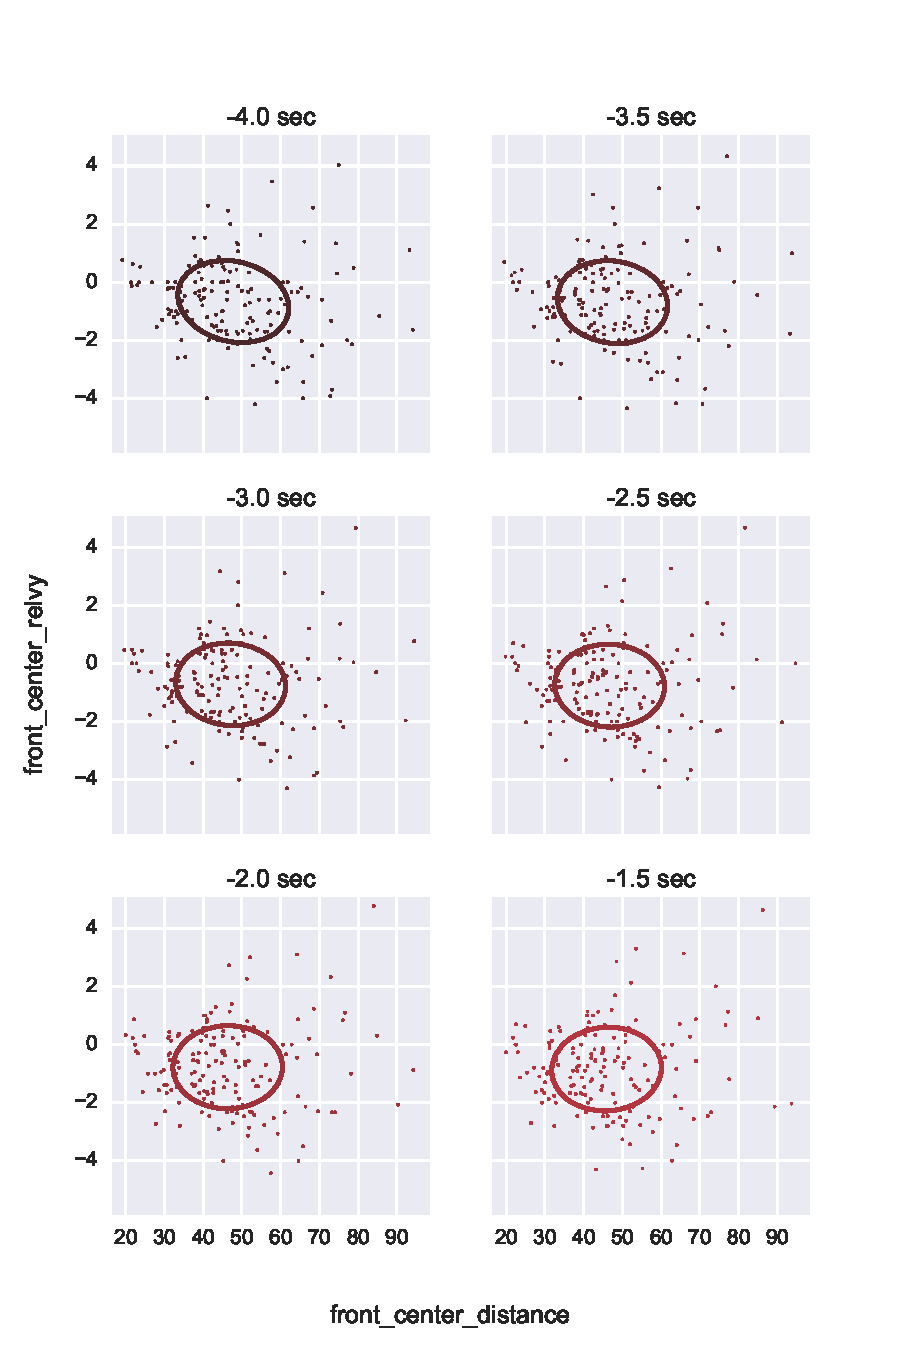
\includegraphics[width=11cm,keepaspectratio]{fig/scatter_ellipse_front_center_distance_front_center_relvy2.pdf}
  % \caption{車線変更開始4秒前から1.5秒前の時点における先行車両との相対距離と相対速度を,すべてのデータにおいてプロットした散布図.また,これを正規分布で近似し,長軸,短軸を標準偏差とした楕円.x軸が距離を,y軸が速度を表す.}
  % \label{fig:scatter_ellipse2}
\end{figure}
\begin{figure}[t]
  \centering
    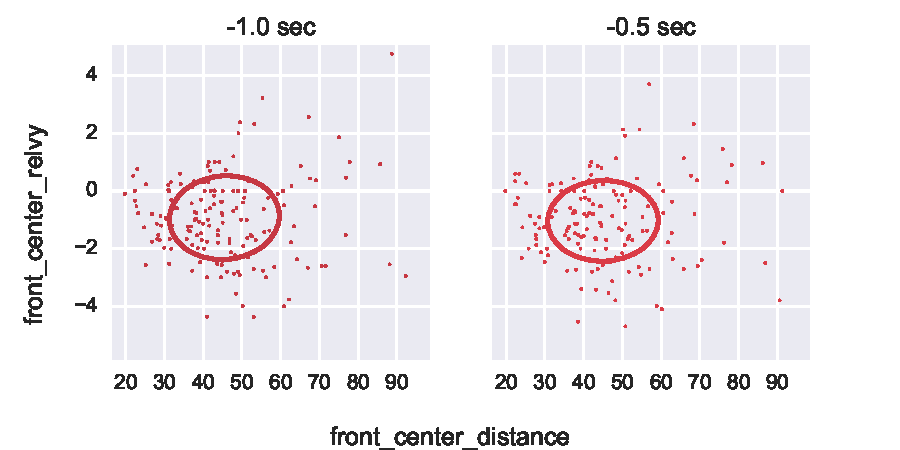
\includegraphics[width=11cm,keepaspectratio]{fig/scatter_ellipse_front_center_distance_front_center_relvy3.pdf}
  \caption{車線変更開始10秒前から0.5秒前の時点における先行車両との相対距離と相対速度を,すべてのデータにおいてプロットした散布図.また,これを正規分布で近似し,長軸,短軸を標準偏差とした楕円.x軸が距離を,y軸が速度を表す.}
  \label{fig:scatter_ellipse}
\end{figure}
